\documentclass[12pt, letterpaper]{article}
\usepackage[utf8]{inputenc}
\usepackage{graphicx}
\usepackage[numbers]{natbib}
\usepackage{amsmath}
\graphicspath{ {images/} }
\title{Deep learning features for COVID-19 screening using Computed Tomography (CT)
scans}
\author{Hugo Morvan}
\date{January 2023}
\begin{document}

\maketitle

\begin{abstract}
%Intro resumé
AI-guided tools can extract distinguish features so lung abnormalities in CT scans can be analyzed. Also, CT scans, according to WHO, are cheaper to use, and therefore, with AI-guided tools, analyzing CT scans for the evidence of COVID-19 can be used in resource-constrained regions. 
%method
In this project, 3D deep learning model (convolutional neural network tailored architecture) was proposed. On a dataset of size 2000 CT scans (publicly available dataset), deep learning models was trained on the USD’s Lawrence Supercomputing Machine: GPU node of the Lawrence consisting of a dual 12-core SkyLake 5000 series CPU, and NVIDIA Tesla V100 32GB CPU and 192GM RAM. 
%results
When limiting to 20 epochs, the performance is promising, which is 65.44\% accuracy on a validation dataset with the lowest possible loss of 0.642.



%discussion

\end{abstract}

\newpage
\section{Acknowledgements}

I would like to express my thanks to my thesis advisor, Dr. KC Santosh, without whom this project would have not started; to Librarian Specialist Kathleen McElhinney for her valuable help in the litterature review and the writting of this thesis. I would also like to thank the University of South Dakota for funding this project through the UDiscover program. Finally, I would like to thank my family and friends for their support and encouragement throughout this project.

\newpage
\tableofcontents

\newpage
\listoffigures

\newpage
\section{Introduction}
%Describe Covid19, in the context of 2022
The novel coronavirus disease SARS-CoV-2 (COVID-19) has spread rapidly and widely since the end of 2019. No country and no community has been spared the direct and indirect impacts of the pandemic \cite{WHO_2021}. It is assumed that when COVID-19 becomes endemic there will be low-level circulation of virus, which underscores the continues importance of public health and social measures even in those countries where vaccination programs are well underway \cite{WHO_2021}\cite{WHO_2022}. The risk of emergence of further variants of concern increases with every instance of transmission. The best way to reduce the risk of further virus mutation is to reduce transmission \cite{WHO_2021}, hence the importance of developing reliable and fast means of detecting the presence of the virus. Currently, diagnostic techniques based on viral RNA amplification, specifically qRT-PCR (quantitative real-time polymerase chain reaction), are the gold standard diagnostic methods for COVID-19 \cite{Teymouri_2021}. However, the RT-PCR test for SARS-CoV-2 virus does have some pitfalls that necessitate improvements in the way the method is used. As with immunodiagnostic tests, the RT-PCR test can have difficulties in distinguishing between true positive and true negative COVID-19 infected individuals, therefore it is a wise precaution not to rely on PCR test results alone, and to consider other clinical and molecular evidence \cite{Teymouri_2021}. 
%Talk about The use of CT-scan to screen covid 19 on patients. 
Chest Computed Tomography (CT) scans can be used as a complementary mean for COVID-19 screening. In a comparative study, \cite{Fang_2020} showed that CT-scans may have a higher sensitivity than RT-PCR. 
%Talk about the use of Deep Learning to improve diagnosis, what is the error rate of technicians ?

%Explain the challenges of it

%Explain the method that will be used in the paper
In this paper, we propose a deep learning model to detect COVID-19 from CT scans whole volume. The model is trained on a dataset of 2000 CT scans. The model is trained on the USD’s Lawrence Supercomputing Machine: GPU node of the Lawrence consisting of a dual 12-core SkyLake 5000 series CPU, and NVIDIA Tesla V100 32GB CPU and 192GM RAM.


\newpage
\section{Related Work}
%Do the lib review here
\subsection{Dataset availability}
Among the publicly available dataset containing CT-scans labeled for COVID-19 classification, 2 categories of datasets emerge: 2D and 3D datasets. 2D datasets are generally images extracted from CT-scans using random slicing (cite), slicing (cite) or manual slicing for significant regions, realised by a physician or a doctor. 3D datasets contains full CT-scans and come in .mha or .dicom file format, as produced by CT-scans machines. In addition to the image data, there is sometimes additional metadata such as age, sex, or other information. The labeling of datasets are realised by physicians and/or utilising one or several RT-PCR tests (cite). One issue with 2D datasets is that it requires the intervention of a physician to select the slices of interest or, if an algorithm is used for the slicing, the risk of missing the area of interest is to consider.Additionally, selecting 2D images from 3D CT-scans results in having numerous images from a single patient and can lead to performance overestimation of models \cite{Altaf_2021}. The problem with using 3D dataset is that it increases the size of the data to be processed and therefore increases the time to train a machine learning model. Since Deep Learning requires large amount of annotated (training) data to learn useful computational models to accurately detect COVID-19 using CT-images \cite{Altaf_2021}, the size of qualitative datasets can get rapidly big.
Talk about the sensitivity of ct scans.  

%Talk about difficulty of finding large dataset, causing researcher to experiment with transfer learning to palliate to the small size datasets of CT-scans. 


\subsection{2-Dimensional Approach}
The literature on COVID-19 detection using chest CT-scans can be divided into 2 categories: the papers where 2-dimensional data is used to train a neural network, and the papers where 3-dimensional data is used to train a neural network.The major challenge of using CT-scans modality for deep learning purposes is that it is a 3-dimensional object, thus it contains a lot of data (compared to other modalities) which can cause to rapidly reach the computing capabilities of a computer / the limits of GPU memory. One strategy to remediated to this problem is to reduce the dimension of the dataset by going from a full (3D) CT-scan to a set of several (2D) CT-scan slices.
%from here the author will be group by preprocessing techniques but the order might change. 

In \cite{Turkoglu_2021}, Turkoglu started with a dataset of 746 CT images then used data augmentation techniques (reflection, rotation) to expand this dataset to 3730 images. Using transfer-learning techniques, the author used a Multiple Kernels-ELM-based Deep Neural Networks (MKs-ELM-DNN) method and obtained an accuracy score of 98.36\% \cite{Turkoglu_2021}.

In \cite{Sen_2021}, Sen et al. used a bi-stage hybrid model to detect COVID-19 from CT images of two different datasets (\cite{Angelov_2020} and \cite{Zhao_2020}). The first stage of this approach is to use a CNN architecture to extract features from the CT images. The second stage is a bi-stage feature selection approach that selects which features to be used for the classification using the Support Vector Machine (SVM) classifier. This method yield a prediction rate of 98.39\% on \cite{Angelov_2020}, and a 90.0\% prediction rate on \cite{Zhao_2020}.

In \cite{Ghassemi_2021}, Ghassemi et al. used pre-trained deep neural networks and a cyclic generative adversarial net (CycleGAN) model for data augmentation. This method reached an accuracy of 99.60\% on a dataset of 189 patients (Iranian hospital). 

In \cite{Aria_2022}, Aria et al. used transfer learning techniques to overcome the problems raised by using small-sized datasets. Their paper proposes an adversarial deep domain adaptation-based approach for diagnosing COVID-19 from lung CT-images, termed ADA-COVID. They achieved an accuracy of 99.96\% on \cite{Angelov_2020}. 

In \cite{Carvalho_2021}, Carvalho et al. used a combination of hyperparameters optimization, feature selection and a multi-layer perceptron classifier to classify images from \cite{Angelov_2020} and \cite{Zhao_2020}. The proposed methodology achieved an accuracy of 99.7\% and 98.7\% on the respective datasets.

In \cite{Jaiswal_2020}, a DenseNet201 based deep transfer learning (DTL) method is proposed by Jaiswal et al. to classify CT images from \cite{Angelov_2020}. The proposed model is utilized to extract features by using its own learned weights on the ImageNet dataset along with a convolutional neural structure to achieve an accuracy of 97\%.

In \cite{Arora_2021}, Arora et al. used transfer learning from existing pre-trained models and a super-residual dense neural network to classify CT images from \cite{Angelov_2020} and \cite{Zhao_2020}. Their method claimed to have achieved a precision of 100\% and 94.12\% respectively.


In \cite{Singh_2021}, Singh and Yow propose an iterpretable deep learning model Ps-ProtoPNet to detect COVID-19 from CT-scan images from \cite{Gunraj_2021}. The highest accuracy that their model achived was 99.29\%.

In \cite{Rahimzadeh_2021}, Rahimzadeh et al. used an image processing algorithm to discard the CT images where the lung is not properly visible in order to reduce processing time and false detection. They used a ResNet50V2 deep neural network on a dataset that they introduced consisting of 48260 CT scan images from 282 normal persons and 15589 images from 95 patients with COVID-19 infections. The proposed method achieved an accuracy of 98.49\% in the single image classification stage, and an accuracy of 95.51\% at the patient identification stage. 

In \cite{Yang_2022}, Yang et al. propose three deep learning architectures, feature-ensemble deep neural network (F-EDNC), fully connected-ensemble deep neural network (FC-EDNC), and output-ensemble deep neural network (O-EDNC) to classify CT images from \cite{Angelov_2020}. The results suggest that the F-EDNC architecture is the best performing architecture with an accuracy of 97.75\%, followed by FC-EDNC and O-EDNC with 97.55\% and 96.12\% accuracy respectively. [Explain what an esemble neural network is later ?]

In \cite{Loey_2020}, Loey et al. used data augmentation techniques along with Conditional Generative Adversarial Networks (CGAN) to generate new images from the dataset of \cite{Zhao_2020}. They used five different deep learning architectures to classify the generated images and achieved best results with the ResNet50 architecture. The authors obtained an accuracy of 82.91\%, a sensitivity of 77.66\% and a specificity of 87.62\%.

In \cite{Alshazly_2020}, Alshazly et al. experimented with twelve different convolutional neural network architectures to classify CT images from the dataset of \cite{Angelov_2020} and \cite{Zhao_2020}. The proposed model achieved average accuracies of 99.4\% and 92.9\%, and sensitivity scores of 99.8\% and 93.7\% on \cite{Angelov_2020} and \cite{Zhao_2020} respectively. The authors also proposed a method to visualize the decision made by the models by using the Grad-CAM technique.

In \cite{Shah_2021}, Shah et al. compared the performances of a self-developed model named CTnet-10 to the performances of several pre-existing CNN architectures in classifying the CT images from \cite{Zhao_2020}. The VGG-19 architecture showed the best results with an accuracy of 94.52\%.

In \cite{Heidari_2022}, Heidari et al. proposed a privacy-aware method for COVID-19 detection in chest CT scans using a lightweight deep neural network, transfer learning, and blockchain technology. The proposed method achived an accuracy of 99.76\% on a combination of 5 different datasets from hospitals in Iran.

\subsection{3-Dimensional Approach}
In this section is presented a list of papers that used 3-dimensional approaches to detect COVID-19 from CT scans. Contrary to the papers in the previous section, these papers do not use 2-dimensional slices of the CT scans, but the whole 3-dimensional volume of the CT scan. 

In \cite{Zhao_2021}, Zhao et al. proposed a new segmentation method, which integrates a 3-dimensional V-Net with a shape deformation module implemented using a spatial transform network (STN). The proposed method achieved an area under the curve (AUC) of 94.70\%, a sensitivity of 96.70\% and a specificity of 92.70\% on a dataset consisting of 112 CT scans, including 58 COVID-19 positive cases and 54 COVID-19 negative cases. Due to the limited size of the dataset, the authors applied data augmentation techniques to increase the size of the dataset, including random flipping, random cropping and random rotation. Rescaling and resampling strategies were also applied to CT scans to overcome the GPU memory limit abd to reduce the computational cost.

In \cite{Pu_2020}

\newpage
\section{Methods}

\subsection{Dataset Description}
For this paper, we consider the STOIC2021 Training dataset. The STOIC project collected Computed Tomography (CT) images of 10,735 individuals suspected of being infected with SARS-COV-2 during the first wave of the pandemic in France, from March to April 2020. For each patient in the training set, the dataset contains binary labels for COVID-19 presence, based on RT-PCR test results, and COVID-19 severity, defined as intubation or death within one month from the acquisition of the CT scan\cite{Revel_2021}. The part of this dataset which is used for this paper is publicly available on AWS Registry of Open Data \cite{STOIC_Training} and consists CT images from 2000 individuals. Each CT-scan is in the dimension of 512*512*(143 - 866) for width*height*depth. The depth value varies from 143 to 866 as each CT-scan has a different amount of layers corresponding to the height of the patient, the mean amount of layers being 433.
\subsection{Pre-processing Methods}

%Talks about the three different preprocessing methods used : low res, high res, slicing.
Pre-processing the dataset before training the deep neural network is necessary as each CT-scan has a different shape. The goal of the pre-processing is therefore to convert each CT-scan into a standardised shape, into a format that is readable by the neural network. First, each CT-scan volume is converted from its original ".mha" file type into a number tensor using the python library Numpy. This allows for the subsequent pre-processing operations to be effectuated. The volume is then normalized to contain values between 0 and 1, 0 being the lowest density in the scan (dark pixels), and 1 being the highest (white pixels). Finally, the volume is resized on all three axis to fit the desired dimensions for the input of the neural network using a zoom function from the SciPy python library and a scaling factor. The scaling factor is calculated as follow : \begin{align}
    Scaling Factor = \frac{Desired Dimension}{Current Dimension}
\end{align}

The input shaped choosen for the experimentation is 128*128*64 as it reduces the size of the dataset to 8Gb, which is small enough to be fitted on a computer GPU.


\subsection{Deep Neural Networks}
In this section, the different deep neural networks used for the experimentation are presented. The first model is a simple 5 layers convolutional neural network, the second model is a ResNet34 architecture, and the third model is a VGG-16 architecture. The models are implemented using the Tensorflow python library.
\subsubsection{Convolutional Neural Network}

%talk about what is a convolutional neural network and why using it for image recognition
%Explain what is Convolution, Batch Normalisation, MaxPooling, Dropouts, padding, activation USING CITATIONS
%Explain why I choose the models I choose
Convolutional Neural Networks are 
\subsubsection{Simple Model}
%The 5 layers CNN

%Explain the architecture of the model
The first architecture used for the experimentation is a simple 5 layers convolutional neural network. The architecture of the model is presented in Figure \ref{fig:CNN}. The model is composed of 5 layers, 3 convolutional layers and 2 fully connected layers. The first convolutional layer has 32 filters of size 3*3*3, the second convolutional layer has 64 filters of size 3*3*3, and the third convolutional layer has 128 filters of size 3*3*3. The first fully connected layer has 128 neurons, and the second fully connected layer has 1 neuron. The activation function used for the convolutional layers is ReLU, and the activation function used for the fully connected layers is sigmoid. The model is implemented using the Tensorflow python library.
\begin{figure}[h]
    \centering
    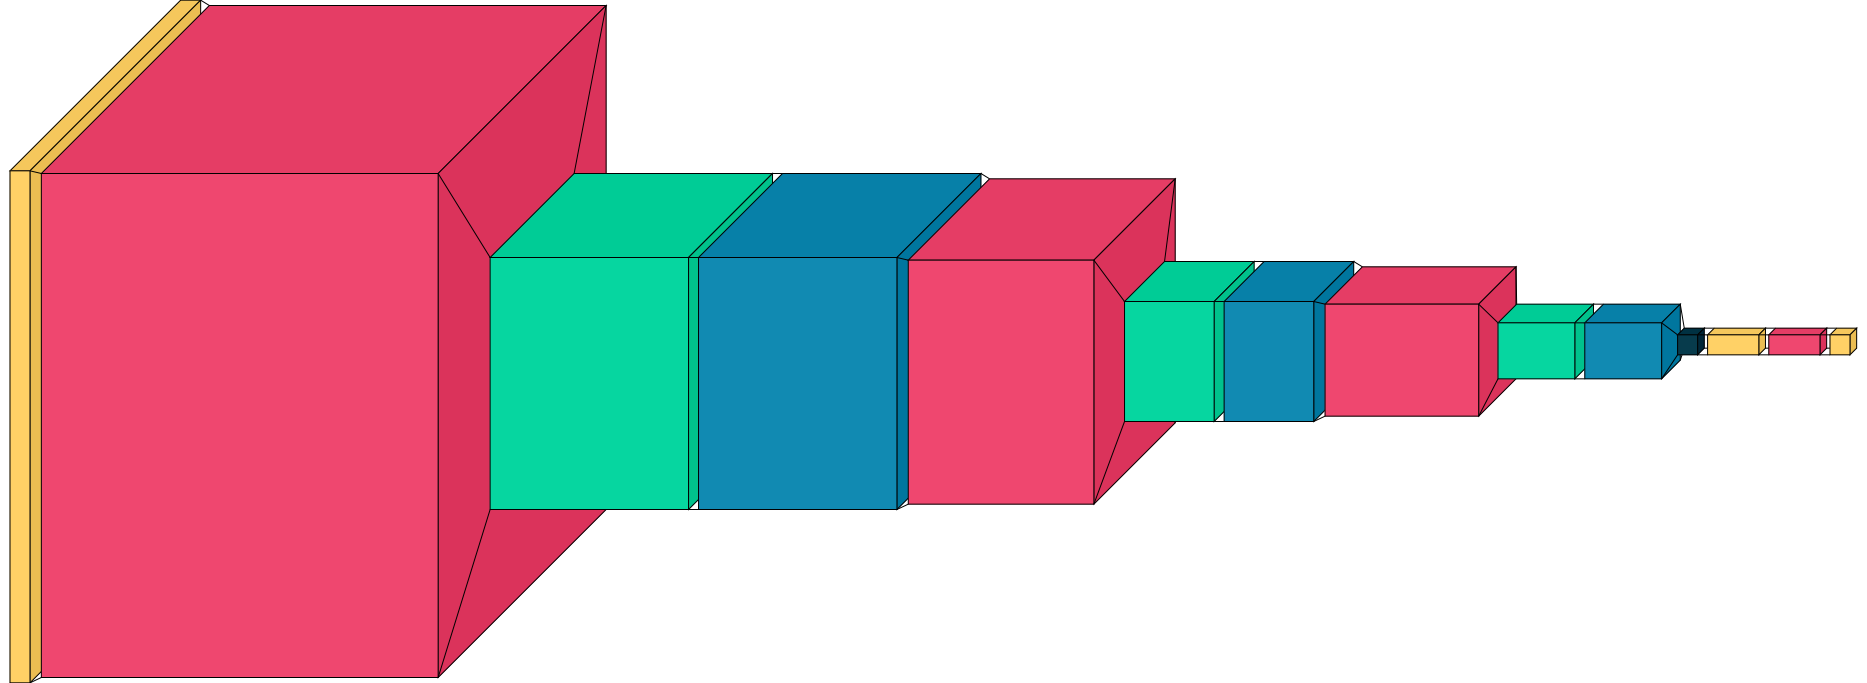
\includegraphics[width=0.8\textwidth]{CNN.png}
    \caption{The architecture of the simple CNN model}
    \label{fig:CNN}
\end{figure}

\subsubsection{ResNet34}
The second architecture used for the experimentation is a ResNet34 architecture. The architecture of the model is presented in Figure \ref{fig:ResNet34}. The model is composed of 5 layers, 3 convolutional layers and 2 fully connected layers. The first convolutional layer has 32 filters of size 3*3*3, the second convolutional layer has 64 filters of size 3*3*3, and the third convolutional layer has 128 filters of size 3*3*3. The first fully connected layer has 128 neurons, and the second fully connected layer has 1 neuron. The activation function used for the convolutional layers is ReLU, and the activation function used for the fully connected layers is sigmoid. The model is implemented using the Tensorflow python library.
\begin{figure}[h]
    \centering
    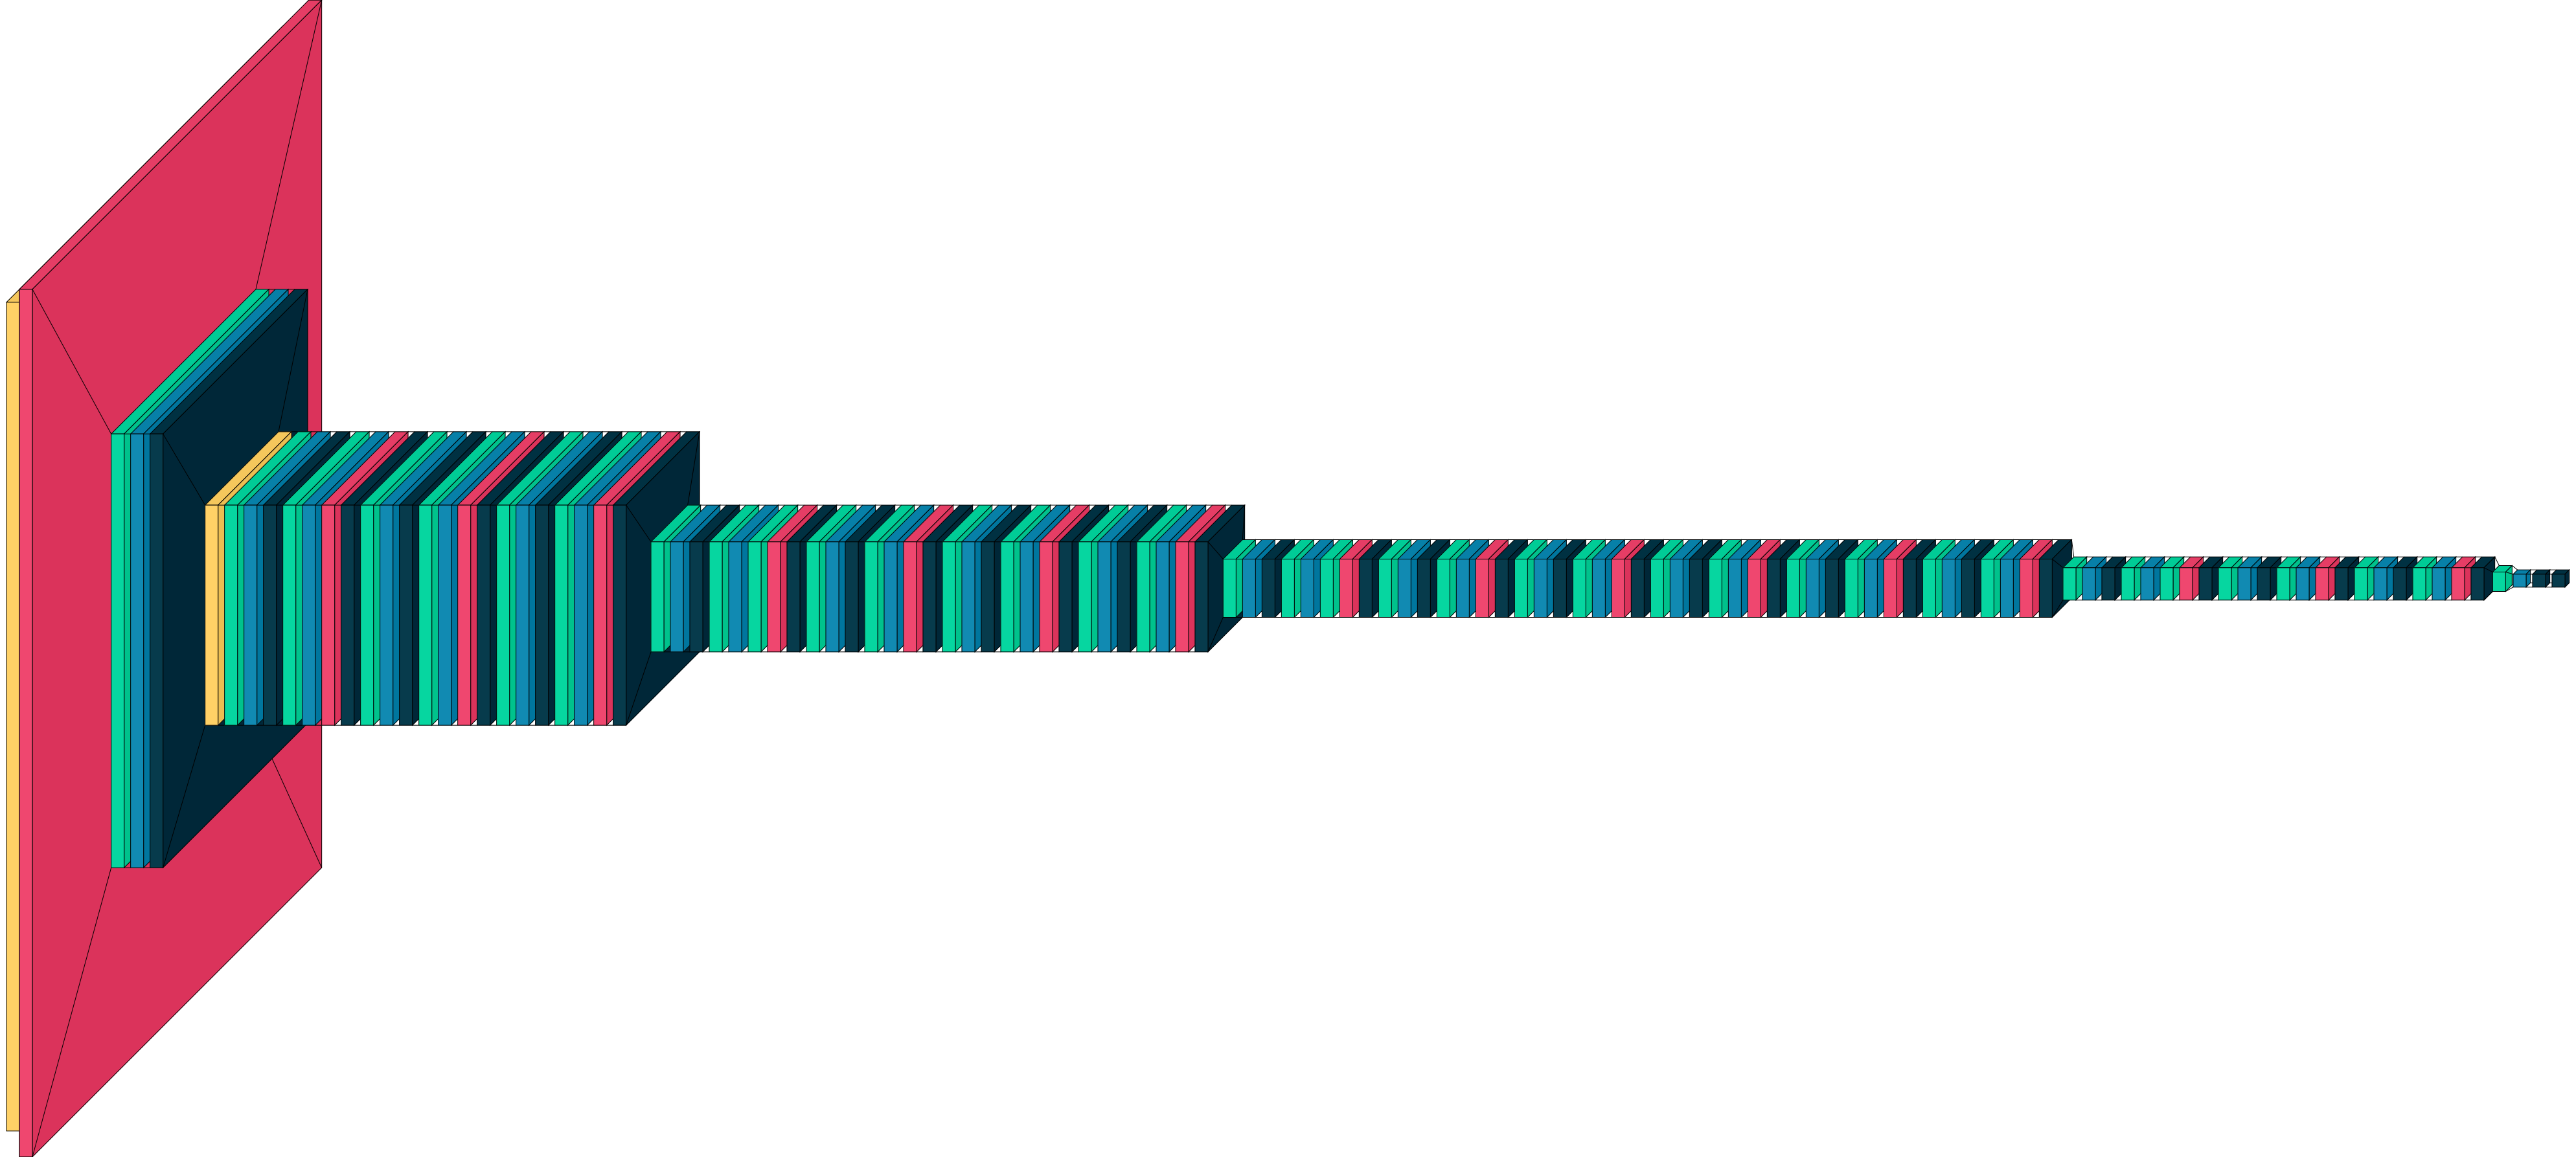
\includegraphics[width=0.8\textwidth]{resnet.png}
    \caption{The architecture of the ResNet34 model}
    \label{fig:ResNet34}
\end{figure}
\subsubsection{VGG-16}
The third architecture used for the experimentation is a VGG-16 architecture. The architecture of the model is presented in Figure \ref{fig:VGG16}. The model is composed of 5 layers, 3 convolutional layers and 2 fully connected layers. The first convolutional layer has 32 filters of size 3*3*3, the second convolutional layer has 64 filters of size 3*3*3, and the third convolutional layer has 128 filters of size 3*3*3. The first fully connected layer has 128 neurons, and the second fully connected layer has 1 neuron. The activation function used for the convolutional layers is ReLU, and the activation function used for the fully connected layers is sigmoid. The model is implemented using the Tensorflow python library.
\begin{figure}[h]
    \centering
    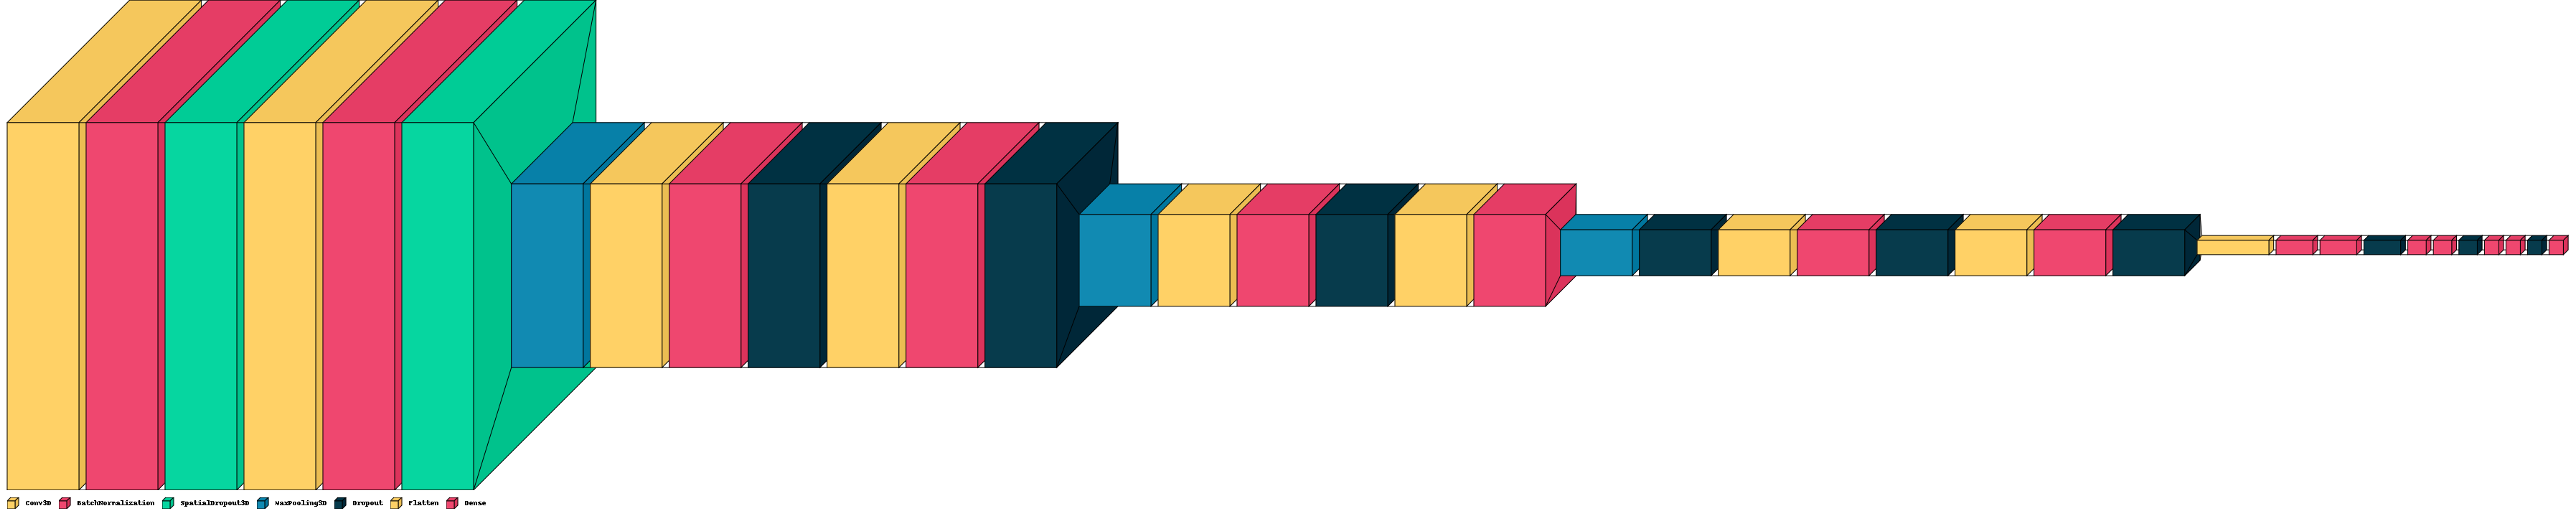
\includegraphics[width=0.8\textwidth]{vgg.png}
    \caption{The architecture of the VGG-16 model}
    \label{fig:VGG16}
\end{figure}

\subsection{Evaluation Metrics}
In this section, the different evaluation metrics used in the litterature to evaluate the performance of the deep neural networks are presented. The first metric is the accuracy, the second metric is the specificity, the third metric is the sensitivity, and the fourth metric is the precision. The metrics are implemented using the Tensorflow python library.
\begin{itemize}
    \item TP : True Positive; designate the amount of CT-scans with a covid+ label correctly identified as covid+ by the model.
    \item FP : False Positive; designate the amount of CT-scans with covid- label incorrectly identified as covid+ by the model.
    \item TN : true negative; designate the amount of CT-scans with a covid- label correctly identified as covid- by the model.
    \item FN : False negative; designate the amount of CT-scans with covid+ label incorrectly identified as covid- by the model.
\end{itemize}

\subsubsection{Accuracy}
Accuracy is the fraction of correctly identified predictions. It measures the overall performance of the model on the test set \cite{Karthik_2021}
\begin{align}
Accuracy = \frac{TP + TN}{TP + FP + FN + TN}
\end{align}

\subsubsection{Specificity}
Specificity measures the proportion of negative class samples that were correctly identified \cite{Karthik_2021}.
\begin{align}
Specificity = \frac{TN}{TN + FP}
\end{align}

\subsubsection{Sensitivity / Recall}
Sensitivity / Recall measures the proportion of positive class samples that were correctly identified \cite{Karthik_2021}.
\begin{align}
    Sensitivity = \frac{TP}{TP + FN}
\end{align}

\subsubsection{Precision}
precision gives the rate of the truly classified positive images among the classes \cite{Karthik_2021}.
\begin{align}
    Precision = \frac{TP}{TP+FP}
\end{align}

\subsubsection{F1-score}
F1 score is a joint of Precision and Recall, expressed as a harmonic mean of this metrics \cite{Karthik_2021}.
\begin{align}
    F1 = 2*\frac{precision*recall}{precision+recall}
\end{align}
%Add recall

\newpage
\section{Experimental Procedure}

\subsection{Dataset separation}

%talks about how the dataset is split in 80\%, 20\% for train, valid
The 2000 CT-scans are split into 80\% for training and 20\% for validation. The validation set is used to evaluate the performance of the model during the training process.

\subsection{Hardware}
%Talk about the use of the Lawrence supercomputer. Explain the reason why this was needed.
As the STOIC2021 dataset containing CT-scans from 2000 patients is relatively large, computation for this project were performed on High Performance Computing systems at the University of South Dakota, funded by NSF Award OAC-1626516. The specific node on which the computations were performed is composed of dual 12-core SkyLake 5000 series CPUs, an Nvidia Tesla 100V 32GB GPU, 192GB of RAM and 240GB SSD. Usage of the Lawrence supercomputer allowed for greatly reduced training times during the experimental phase of this research. USD research Computing staff Bill Cone provided valuable technical expertise and assistance to this project.


\subsection{Training parameters}
%Explain what were the parameters used for the training : epochs, early stopping, loss function, optimizer, batch size, metrics measured
The training phase of this research was divided into two phases. The first phase was the experimental phase, where different architectures were tested and compared. The second phase was the final phase, where the best performing architecture was trained for 20 epochs.

During the experimental phase, the following parameters were used to obtain a first set of results :
\begin{itemize}
    \item Epochs : 50
    \item Loss Function : Binary Cross Entropy
    \item Optimizer : Adam
    \item Batch Size : 16
    \item Metrics : Accuracy, Loss
\end{itemize}

After determining the best performing architecture, the final phase of the training was performed.
The following parameters were used to obtained the results presented in this paper :
\begin{itemize}
    \item Epochs : 20
    \item Loss Function : Binary Cross Entropy
    \item Optimizer : Adam
    \item Batch Size : 16
    \item Metrics : Accuracy, Loss
\end{itemize}

\newpage
\section{Results}

\subsection{Experimental phase}

\subsection{Final phase}
%add the graphs, tables with values, accuracy, loss, specificity, what it means in the context of diagnosing patients.
After training the Convolutional Neural Network for 20 epochs, the accuracy reached a maximum of 63\% on the validation set and 65.4\% on the training set while the loss reached its lowest at 0.644 for the validation set and 0.642 for the training set. 

\newpage
\section{Discussion}
%unpack the results


\newpage
\section{Conclusions and Future Work}
The accuracy of this model in detecting the presence of COVID-19 on CT-scans shows that Deep Learning models can be useful tools for mass screening. Deep learning tools could in this case facilitate the triage of COVID-19 and nonCOVID-19 patients, and thus improve diagnosis on thoracic symptoms as well as limit the spread of the most contagious virus. In the future, this project could be combined with other well-known deep learning models trained on different image data types such as chest x-rays to employ multimodal learning and representation for COVID-19 screening. This could possibly provide more information in detecting anomaly patterns due to COVID-19. Further research could also try to improve the performances of this project by using a higher-resolution preprocessed data or by experimenting with data augmentation techniques.

\newpage
\bibliographystyle{IEEEtranN}
\bibliography{refs.bib}
\nocite{*}

\end{document}